\documentclass[]{article}
\usepackage{lmodern}
\usepackage{amssymb,amsmath}
\usepackage{ifxetex,ifluatex}
\usepackage{fixltx2e} % provides \textsubscript
\ifnum 0\ifxetex 1\fi\ifluatex 1\fi=0 % if pdftex
  \usepackage[T1]{fontenc}
  \usepackage[utf8]{inputenc}
\else % if luatex or xelatex
  \ifxetex
    \usepackage{mathspec}
  \else
    \usepackage{fontspec}
  \fi
  \defaultfontfeatures{Ligatures=TeX,Scale=MatchLowercase}
\fi
% use upquote if available, for straight quotes in verbatim environments
\IfFileExists{upquote.sty}{\usepackage{upquote}}{}
% use microtype if available
\IfFileExists{microtype.sty}{%
\usepackage{microtype}
\UseMicrotypeSet[protrusion]{basicmath} % disable protrusion for tt fonts
}{}
\usepackage[margin=1in]{geometry}
\usepackage{hyperref}
\hypersetup{unicode=true,
            pdftitle={How to SWAP questions' codes with questions' labels from SPSS files in R},
            pdfauthor={Author: Wisner CELUCUS},
            pdfborder={0 0 0},
            breaklinks=true}
\urlstyle{same}  % don't use monospace font for urls
\usepackage{color}
\usepackage{fancyvrb}
\newcommand{\VerbBar}{|}
\newcommand{\VERB}{\Verb[commandchars=\\\{\}]}
\DefineVerbatimEnvironment{Highlighting}{Verbatim}{commandchars=\\\{\}}
% Add ',fontsize=\small' for more characters per line
\usepackage{framed}
\definecolor{shadecolor}{RGB}{248,248,248}
\newenvironment{Shaded}{\begin{snugshade}}{\end{snugshade}}
\newcommand{\AlertTok}[1]{\textcolor[rgb]{0.94,0.16,0.16}{#1}}
\newcommand{\AnnotationTok}[1]{\textcolor[rgb]{0.56,0.35,0.01}{\textbf{\textit{#1}}}}
\newcommand{\AttributeTok}[1]{\textcolor[rgb]{0.77,0.63,0.00}{#1}}
\newcommand{\BaseNTok}[1]{\textcolor[rgb]{0.00,0.00,0.81}{#1}}
\newcommand{\BuiltInTok}[1]{#1}
\newcommand{\CharTok}[1]{\textcolor[rgb]{0.31,0.60,0.02}{#1}}
\newcommand{\CommentTok}[1]{\textcolor[rgb]{0.56,0.35,0.01}{\textit{#1}}}
\newcommand{\CommentVarTok}[1]{\textcolor[rgb]{0.56,0.35,0.01}{\textbf{\textit{#1}}}}
\newcommand{\ConstantTok}[1]{\textcolor[rgb]{0.00,0.00,0.00}{#1}}
\newcommand{\ControlFlowTok}[1]{\textcolor[rgb]{0.13,0.29,0.53}{\textbf{#1}}}
\newcommand{\DataTypeTok}[1]{\textcolor[rgb]{0.13,0.29,0.53}{#1}}
\newcommand{\DecValTok}[1]{\textcolor[rgb]{0.00,0.00,0.81}{#1}}
\newcommand{\DocumentationTok}[1]{\textcolor[rgb]{0.56,0.35,0.01}{\textbf{\textit{#1}}}}
\newcommand{\ErrorTok}[1]{\textcolor[rgb]{0.64,0.00,0.00}{\textbf{#1}}}
\newcommand{\ExtensionTok}[1]{#1}
\newcommand{\FloatTok}[1]{\textcolor[rgb]{0.00,0.00,0.81}{#1}}
\newcommand{\FunctionTok}[1]{\textcolor[rgb]{0.00,0.00,0.00}{#1}}
\newcommand{\ImportTok}[1]{#1}
\newcommand{\InformationTok}[1]{\textcolor[rgb]{0.56,0.35,0.01}{\textbf{\textit{#1}}}}
\newcommand{\KeywordTok}[1]{\textcolor[rgb]{0.13,0.29,0.53}{\textbf{#1}}}
\newcommand{\NormalTok}[1]{#1}
\newcommand{\OperatorTok}[1]{\textcolor[rgb]{0.81,0.36,0.00}{\textbf{#1}}}
\newcommand{\OtherTok}[1]{\textcolor[rgb]{0.56,0.35,0.01}{#1}}
\newcommand{\PreprocessorTok}[1]{\textcolor[rgb]{0.56,0.35,0.01}{\textit{#1}}}
\newcommand{\RegionMarkerTok}[1]{#1}
\newcommand{\SpecialCharTok}[1]{\textcolor[rgb]{0.00,0.00,0.00}{#1}}
\newcommand{\SpecialStringTok}[1]{\textcolor[rgb]{0.31,0.60,0.02}{#1}}
\newcommand{\StringTok}[1]{\textcolor[rgb]{0.31,0.60,0.02}{#1}}
\newcommand{\VariableTok}[1]{\textcolor[rgb]{0.00,0.00,0.00}{#1}}
\newcommand{\VerbatimStringTok}[1]{\textcolor[rgb]{0.31,0.60,0.02}{#1}}
\newcommand{\WarningTok}[1]{\textcolor[rgb]{0.56,0.35,0.01}{\textbf{\textit{#1}}}}
\usepackage{graphicx,grffile}
\makeatletter
\def\maxwidth{\ifdim\Gin@nat@width>\linewidth\linewidth\else\Gin@nat@width\fi}
\def\maxheight{\ifdim\Gin@nat@height>\textheight\textheight\else\Gin@nat@height\fi}
\makeatother
% Scale images if necessary, so that they will not overflow the page
% margins by default, and it is still possible to overwrite the defaults
% using explicit options in \includegraphics[width, height, ...]{}
\setkeys{Gin}{width=\maxwidth,height=\maxheight,keepaspectratio}
\IfFileExists{parskip.sty}{%
\usepackage{parskip}
}{% else
\setlength{\parindent}{0pt}
\setlength{\parskip}{6pt plus 2pt minus 1pt}
}
\setlength{\emergencystretch}{3em}  % prevent overfull lines
\providecommand{\tightlist}{%
  \setlength{\itemsep}{0pt}\setlength{\parskip}{0pt}}
\setcounter{secnumdepth}{0}
% Redefines (sub)paragraphs to behave more like sections
\ifx\paragraph\undefined\else
\let\oldparagraph\paragraph
\renewcommand{\paragraph}[1]{\oldparagraph{#1}\mbox{}}
\fi
\ifx\subparagraph\undefined\else
\let\oldsubparagraph\subparagraph
\renewcommand{\subparagraph}[1]{\oldsubparagraph{#1}\mbox{}}
\fi

%%% Use protect on footnotes to avoid problems with footnotes in titles
\let\rmarkdownfootnote\footnote%
\def\footnote{\protect\rmarkdownfootnote}

%%% Change title format to be more compact
\usepackage{titling}

% Create subtitle command for use in maketitle
\newcommand{\subtitle}[1]{
  \posttitle{
    \begin{center}\large#1\end{center}
    }
}

\setlength{\droptitle}{-2em}

  \title{How to SWAP questions' codes with questions' labels from SPSS files in R}
    \pretitle{\vspace{\droptitle}\centering\huge}
  \posttitle{\par}
    \author{Author: Wisner CELUCUS}
    \preauthor{\centering\large\emph}
  \postauthor{\par}
      \predate{\centering\large\emph}
  \postdate{\par}
    \date{March 11, 2020}


\begin{document}
\maketitle

\hypertarget{useful-for-sharing-spss-.sav-file-on-excel-or-csv-format.}{%
\subsubsection{Useful for sharing SPSS (.sav) file on Excel or CSV
format.}\label{useful-for-sharing-spss-.sav-file-on-excel-or-csv-format.}}

This is a very quick way to read a .sav file and swap the question codes
with the question labels. That can be useful if you want to share an
SPSS survey file with someone who doesn't have SPSS on his PC.

\hypertarget{why-this-matters}{%
\subsubsection{Why this matters?}\label{why-this-matters}}

\textbf{story time}

I recently received an SPSS file (.sav) from a friend for some analysis.
Since I do not have an SPSS on my PC, I had to use my good friend, R, to
read it. I then google the famous ``how to read a .sav file in R''. I
came up with some blog posts that explained how to read the file but
with no additional warning on possible issues with questions' labels.

Once I knew how to read the file, it looked like a straightforward task
for me and I thought R was going to easily ingest the dataset and I'd be
able to do the analysis. I was wrong and disappointed when I realized
the first row of the returned DataFrame did not contain the questions
labels but the questions' codes.

I confirmed there were questions labels by viewing the meta structure of
the DataFrame. Now that, I had the confirmation, the next milestone was
to have the questions' codes replaced by the questions' labels so that
the dataset can be human-readable and nicely organized to be shared on
CSV or XLSX format.

I sought on the internet, visited many blogs and watched Youtube videos,
I could not find an adequate solution. So, I went to the foreign package
documentation, the solution was there but not so obvious. I spent some
time figuring out how to use the package to capture the questions'
labels and at the end swap them with the questions' code. Finally, I was
able to find a solution to the issue.

\textbf{The moral of the story}

You may be in the position of the one that will receive or the one that
will share a data set from SPSS software but can't manage to export a
proper CSV or Excel file for your client.

You never know, some people may be searching desperately a solution for
a similar problem just like I was. Hopefully, if they come across this
article, it will save them some time.

\textbf{First install and upload the foreign package}

The package used to read the SPSS file in R is the \textbf{foreign}
package. This package has a useful \textbf{read.spss} function to ingest
the .sav file provided by the SPSS software.

\begin{Shaded}
\begin{Highlighting}[]
\CommentTok{#install.packages("foreign") }
\CommentTok{## uncomment the line above to install the foreign package if it is not pre-installed in your PC.}

\KeywordTok{library}\NormalTok{(foreign) }\CommentTok{#load the package}
\end{Highlighting}
\end{Shaded}

\hypertarget{read-the-sav-file-using-the-read.spss-function-from-the-foreign-package.}{%
\subsubsection{Read the sav file using the read.spss function from the
foreign
package.}\label{read-the-sav-file-using-the-read.spss-function-from-the-foreign-package.}}

For this demonstration, I am using a dataset from the
\href{http://spss.allenandunwin.com.s3-website-ap-southeast-2.amazonaws.com/data-files.html\#.XmlmC6hKjIU}{web
page}. Credit goes to the page author for making the dataset availlable
for us.

If you want to try the solution with the same dataset, click on:
\href{http://spss.allenandunwin.com.s3-website-ap-southeast-2.amazonaws.com/Files/sleep.zip}{download}.

Let's now read the file:

\begin{Shaded}
\begin{Highlighting}[]
\NormalTok{dataset <-}\StringTok{ }\KeywordTok{read.spss}\NormalTok{(}\StringTok{"./sleep.sav"}\NormalTok{, }\DataTypeTok{to.data.frame =} \OtherTok{TRUE}\NormalTok{)}

\CommentTok{#Use file.choose() to graphically attached the file to the read.spss function if your not comfortable writing path to file manually. }
\CommentTok{#dataset <- read.spss(file.choose(), to.data.frame = TRUE)}

\KeywordTok{head}\NormalTok{(dataset[}\DecValTok{1}\OperatorTok{:}\DecValTok{7}\NormalTok{])}
\end{Highlighting}
\end{Shaded}

\begin{verbatim}
##    id    sex age         marital              edlevel weight height
## 1  83 female  42 married/defacto     secondary school     52    162
## 2 294 female  54 married/defacto  postgraduate degree     65    174
## 3 425   male  NA married/defacto     secondary school     89    170
## 4  64 female  41 married/defacto  postgraduate degree     66    178
## 5 536 female  39 married/defacto  postgraduate degree     62    160
## 6  57 female  66 married/defacto undergraduate degree     62    165
\end{verbatim}

The first 5 lines of the first 7 columns of the dataset show the
columns' names. But they are not useful as they do not allow us to
understand what the columns' values are about.

Be aware that SPSS gathers the survey responses in a specific tab, and
in additional tabs you can read the question labels and the question
values for single or multiple choice questions when using the software.
Now, in R, we only obtain the questions code. That is not so useful if
we want to save this dataset as CSV to share with friends. We will
correct that.

\textbf{Let's confirm that the file contains questions' labels}

\begin{Shaded}
\begin{Highlighting}[]
\KeywordTok{View}\NormalTok{(dataset)}
\end{Highlighting}
\end{Shaded}

By executing this command, R studio will open a new tab with a table
showing the questions' codes associated with the questions' labels. See
the following picture:

\begin{figure}
\centering
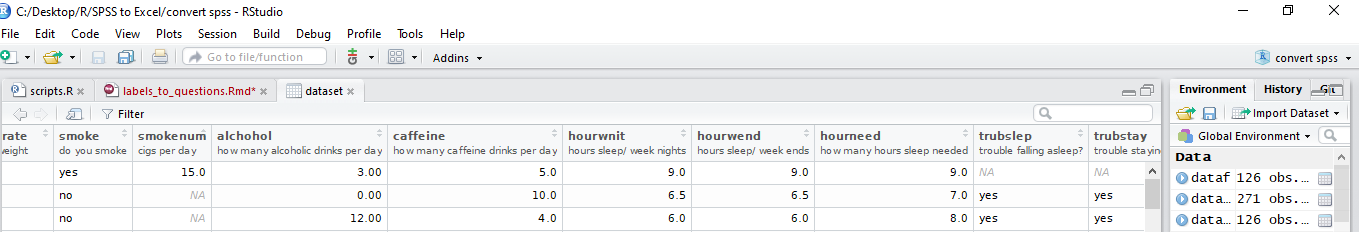
\includegraphics{./picture.png}
\caption{Data with questions' labels}
\end{figure}

\hypertarget{how-to-access-the-questions-labels-in-r.}{%
\subsubsection{How to access the questions' labels in
R?.}\label{how-to-access-the-questions-labels-in-r.}}

As I mentioned in the story, I found a way to access the questions'
labels thanks to the \textbf{foreign} package \textbf{read.spss}
documention
\href{https://www.rdocumentation.org/packages/foreign/versions/0.8-75/topics/read.spss}{here}.

In the detail section of te documention, one can read this: ``If SPSS
variable labels are present, they are returned as the''variable.labels"
attribute of the answer". Very clear, right?

If that is esoteric for you, play with the \textbf{to.data.frame}
parameter by setting it to \emph{FALSE}. You will notice that
\textbf{variable.labels} is truly an element of the list returning by
the function call. As an attribute of the results object, we can
directly extract it by calling the attributes() function on the results'
object.

\begin{Shaded}
\begin{Highlighting}[]
\KeywordTok{library}\NormalTok{(dplyr) }\CommentTok{#load it to use glimpse()}

\NormalTok{results <-}\StringTok{ }\KeywordTok{read.spss}\NormalTok{(}\StringTok{"./sleep.sav"}\NormalTok{, }\DataTypeTok{to.data.frame =} \OtherTok{FALSE}\NormalTok{)}

\CommentTok{#class(results) # Show the class of results, a list indeed.}
\CommentTok{#glimpse(attr(data, "variable.labels")) #show brief description of each attributes of the elements of the list.}

\CommentTok{#length(attributes(results)$variable.labels) # confirm the number of labels.}
\KeywordTok{attributes}\NormalTok{(results)}\OperatorTok{$}\NormalTok{variable.labels[}\KeywordTok{c}\NormalTok{(}\DecValTok{1}\OperatorTok{:}\DecValTok{5}\NormalTok{)] }\CommentTok{# show the first 5 elements of the named vector.}
\end{Highlighting}
\end{Shaded}

\begin{verbatim}
##                                 id                                sex 
##            "Identification Number"                              "sex" 
##                                age                            marital 
##                              "age"                   "marital status" 
##                            edlevel 
## "highest education level achieved"
\end{verbatim}

Now that we have the list of the labels, we can proceed. But, we won't
be able to just read it now, we need to first extract the labels because
they are still attached to the questions' codes. In fact, the returning
data structure of the previous lines of code is a named vector where
each vector member is assigned a name which is a question code. Let's
convert and store the named vector in a DataFrame variable.

\begin{Shaded}
\begin{Highlighting}[]
\NormalTok{results.labels =}\StringTok{ }\KeywordTok{as.data.frame}\NormalTok{(}\KeywordTok{attributes}\NormalTok{(results)}\OperatorTok{$}\NormalTok{variable.labels)}

\CommentTok{#Print the five first rows}
\KeywordTok{head}\NormalTok{(results.labels)}
\end{Highlighting}
\end{Shaded}

\begin{verbatim}
##         attributes(results)$variable.labels
## id                    Identification Number
## sex                                     sex
## age                                     age
## marital                      marital status
## edlevel    highest education level achieved
## weight
\end{verbatim}

Nice! let's rename the column ``attributes(results)\$variable.labels''

\begin{Shaded}
\begin{Highlighting}[]
\KeywordTok{names}\NormalTok{(results.labels) <-}\StringTok{ "labels"}


\KeywordTok{head}\NormalTok{(results.labels)}
\end{Highlighting}
\end{Shaded}

\begin{verbatim}
##                                   labels
## id                 Identification Number
## sex                                  sex
## age                                  age
## marital                   marital status
## edlevel highest education level achieved
## weight
\end{verbatim}

Perfect. We can now simply extract the columns labels in a character
vector.

\begin{Shaded}
\begin{Highlighting}[]
\NormalTok{labels <-}\StringTok{ }\KeywordTok{as.character}\NormalTok{(results.labels}\OperatorTok{$}\NormalTok{labels) }
\NormalTok{labels[}\DecValTok{1}\OperatorTok{:}\DecValTok{10}\NormalTok{]}
\end{Highlighting}
\end{Shaded}

\begin{verbatim}
##  [1] "Identification Number"            "sex"                             
##  [3] "age"                              "marital status"                  
##  [5] "highest education level achieved" ""                                
##  [7] ""                                 "general health"                  
##  [9] "physical fitness"                 "current weight"
\end{verbatim}

\hypertarget{lets-start-swapping-finally}{%
\subsubsection{Let's start swapping
finally!!!}\label{lets-start-swapping-finally}}

Since we manage to extract the labels of the questions. We can swap them
with the questions' codes now and rename the columns' names, and lastly
save it for sharing with humans who do not have SPSS!

\textbf{Why do we need to swap instead of just replace the questions'
codes by the labels?}

If you are still following and is an intermediate R user, you may be
asking the above question. Here is the answer. We need to swap because
not all the questions' codes have a matching label! So, we need to make
sure we don't replace questions' codes with empty strings. If a
question's code is not associated with a label, we won't swap it and
keep it in place. So, now we are agreed, right? let's continue!

Remember, earlier we read the data from the .sav file and saved it in
\textbf{dataset} variable as a DataFrame by setting
\textbf{to.data.frame} of the \textbf{read.spss} function to
\textbf{TRUE}.

Now we will write a function that will take the question codes and the
labels as parameters and swap them whenever possible.

\begin{Shaded}
\begin{Highlighting}[]
\NormalTok{swap_qc_l <-}\StringTok{ }\ControlFlowTok{function}\NormalTok{(q_codes, q_labels)\{}
\NormalTok{  questions <-}\StringTok{ }\KeywordTok{character}\NormalTok{()}
  
  \CommentTok{#Test if the vectors are on the same length. if they are not, big trouble!}
\NormalTok{  assertthat}\OperatorTok{::}\KeywordTok{are_equal}\NormalTok{(}\KeywordTok{length}\NormalTok{(q_codes), }\KeywordTok{length}\NormalTok{(q_labels))  }
  \ControlFlowTok{for}\NormalTok{(i }\ControlFlowTok{in} \DecValTok{1}\OperatorTok{:}\KeywordTok{length}\NormalTok{(q_codes))\{}
    \ControlFlowTok{if}\NormalTok{(q_labels[i] }\OperatorTok{==}\StringTok{ ""}\NormalTok{)\{}
\NormalTok{      questions[i] =}\StringTok{ }\NormalTok{q_codes[i]}
\NormalTok{    \}}\ControlFlowTok{else}\NormalTok{\{}
\NormalTok{      questions[i] =}\StringTok{ }\NormalTok{q_labels[i]}
\NormalTok{    \}}
\NormalTok{  \}}
  \KeywordTok{return}\NormalTok{(questions)}
\NormalTok{\}}
\end{Highlighting}
\end{Shaded}

\textbf{We can call the function now}.

\begin{Shaded}
\begin{Highlighting}[]
\NormalTok{question_codes <-}\StringTok{ }\KeywordTok{as.character}\NormalTok{(}\KeywordTok{colnames}\NormalTok{(dataset)) }\CommentTok{#First extract questions' codes. first row of the DataFrame dataset.}

\NormalTok{questions <-}\StringTok{ }\KeywordTok{swap_qc_l}\NormalTok{(question_codes,labels)}

\KeywordTok{colnames}\NormalTok{(dataset) <-}\StringTok{ }\NormalTok{questions}
\KeywordTok{head}\NormalTok{(dataset[}\DecValTok{1}\OperatorTok{:}\DecValTok{7}\NormalTok{])}
\end{Highlighting}
\end{Shaded}

\begin{verbatim}
##   Identification Number    sex age  marital status
## 1                    83 female  42 married/defacto
## 2                   294 female  54 married/defacto
## 3                   425   male  NA married/defacto
## 4                    64 female  41 married/defacto
## 5                   536 female  39 married/defacto
## 6                    57 female  66 married/defacto
##   highest education level achieved weight height
## 1                 secondary school     52    162
## 2              postgraduate degree     65    174
## 3                 secondary school     89    170
## 4              postgraduate degree     66    178
## 5              postgraduate degree     62    160
## 6             undergraduate degree     62    165
\end{verbatim}

Voila! If you want to be sure that there was no error in swapping
vectors, you can call \textbf{View()} again with \textbf{dataset} as an
argument to see if the labels swapped match the preset ones.

\begin{Shaded}
\begin{Highlighting}[]
\CommentTok{#View(dataset)}
\end{Highlighting}
\end{Shaded}

Thank you for reading, don't forget to share in your network to help
others.

Peace!


\end{document}
